\hypertarget{arrivuxe9e-dans-lempire-du-milieu}{%
\section{Arrivée dans l'empire du
milieu}\label{arrivuxe9e-dans-lempire-du-milieu}}

\emph{Lundi 11 juin 2018}

C'est au terme d'une correspondance ratée (mais reroutée avec brio par
China Southern Airlines, au prix d'une course à travers tout l'aéroport
de Wuhan) que nous sommes arrivés à Shanghai.

Nous y avons eu le plaisir de passer deux soirées avec Longhui et Chen
qui, en tant que bons connaisseurs de la France, nous ont expliqué
quelques fondamentaux sur la Chine.

\begin{figure}
\centering
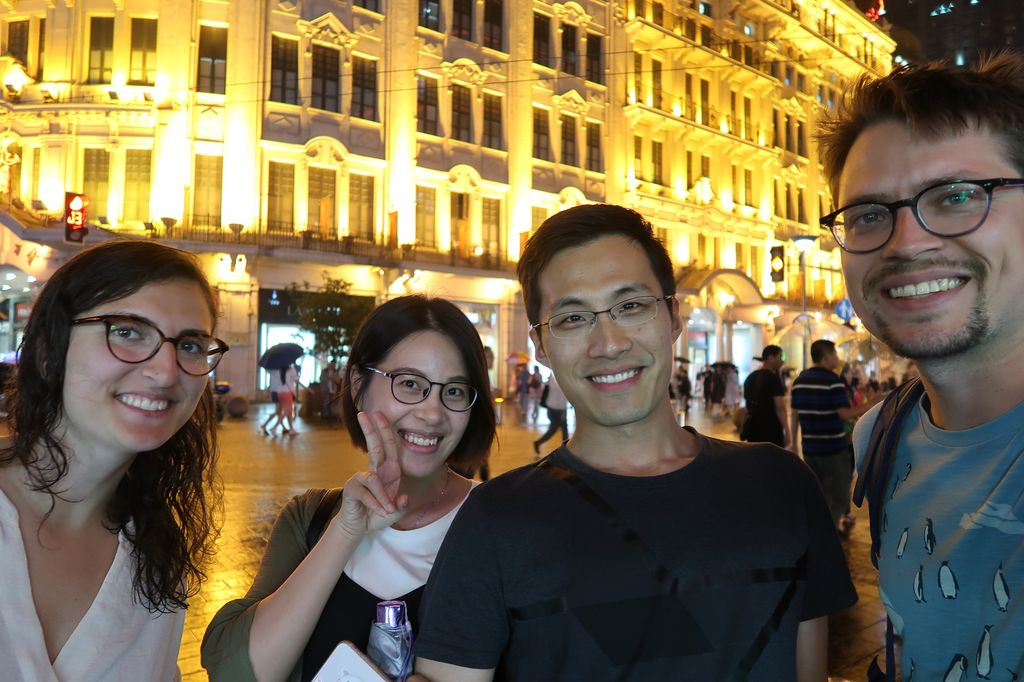
\includegraphics{images/20180611_shanghai.JPG}
\caption{Selfie 'classique' dans la rue piétonne Nanjing Road, près du
Bund.}
\end{figure}

Nous avons ensuite admiré la vue depuis la promenade du Bund, sur les
berges du fleuve Huangpu.

\begin{figure}
\centering
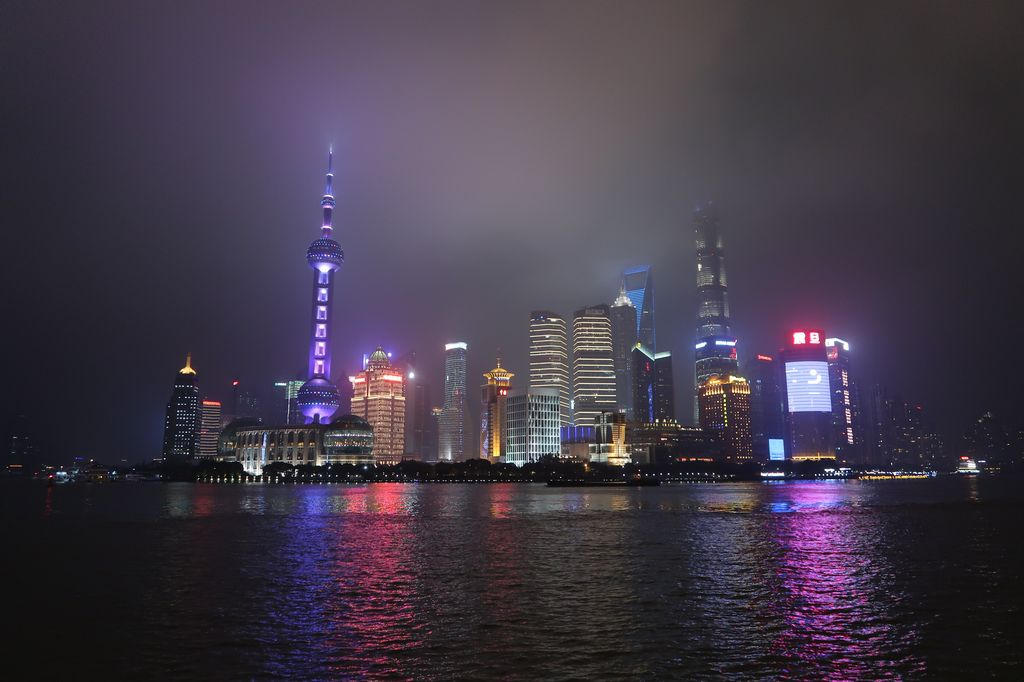
\includegraphics{images/20180611_bund.JPG}
\caption{La vue sur les gratte-ciels de la nouvelle ville de Shanghai,
Pudong.}
\end{figure}

Tout ceci augure de belles découvertes pour notre tour de la Chine dans
les deux prochaines semaines !

\emph{Florian et Elida}

\hypertarget{commentaires}{%
\subsection{Commentaires}\label{commentaires}}

\begin{itemize}
\item
  pythux, \emph{2018-06-25 20h47}

  Heureux d'apprendre que vous n'y êtes pas arrivé à pieds!
\item
  Florian LB, \emph{2018-07-10 03h50}

  Puisqu'on te dit qu'on est arrivés en avion... :-D
\end{itemize}

